\section{System Architecture}
\label{sec:system-architecture}

On a very high level, \system can be viewed as a three component system:

\begin{itemize}
    \item \textbf{A network of pub/sub nodes, }clustered into efficient overlays, one per topic, for topic-based event dissemination.
    Small overlays, with efficient routing paths satisfy the \emph{high dissemination speed} requirement.
    \item \textbf{A network of replication servers, }tightly connected to each other to facilitate rapid event retrieval and
    prompt maintenance.
    This component is responsible for \emph{event persistence}, and \emph{reliability} allowing nodes to retrieve lost events at any time.
    \item \textbf{Two Cardano smart contracts. }To facilitate authentication and access control for both networks in a decentralized fashion,
    we introduce a blockchain component, in the form of two smart contracts.
    The first serves as a global Topic Registry, maintaining topic configurations and enforcing administrative permissions, thereby satisfying the \emph{authorization and access control} requirement.
    The second manages the registration and membership of replication servers.
\end{itemize}

The event-dissemination network creation protocol is designed such that, regardless of the number of nodes, whether thousands or hundreds of thousands,
the same constant number of communications is required in order to establish topic communication.
Topic discovery requires only a simple lookup operation in the Topic Registry.
Thus, the \emph{scalability} requirement is satisfied.

\subsection{Publisher/Subscriber Network}
\label{subsec:publisher/subscriber-network}

\begin{figure}
    \centering
    \hspace*{-0.5cm}
    \begin{minipage}{0.50\textwidth}
        \centering
        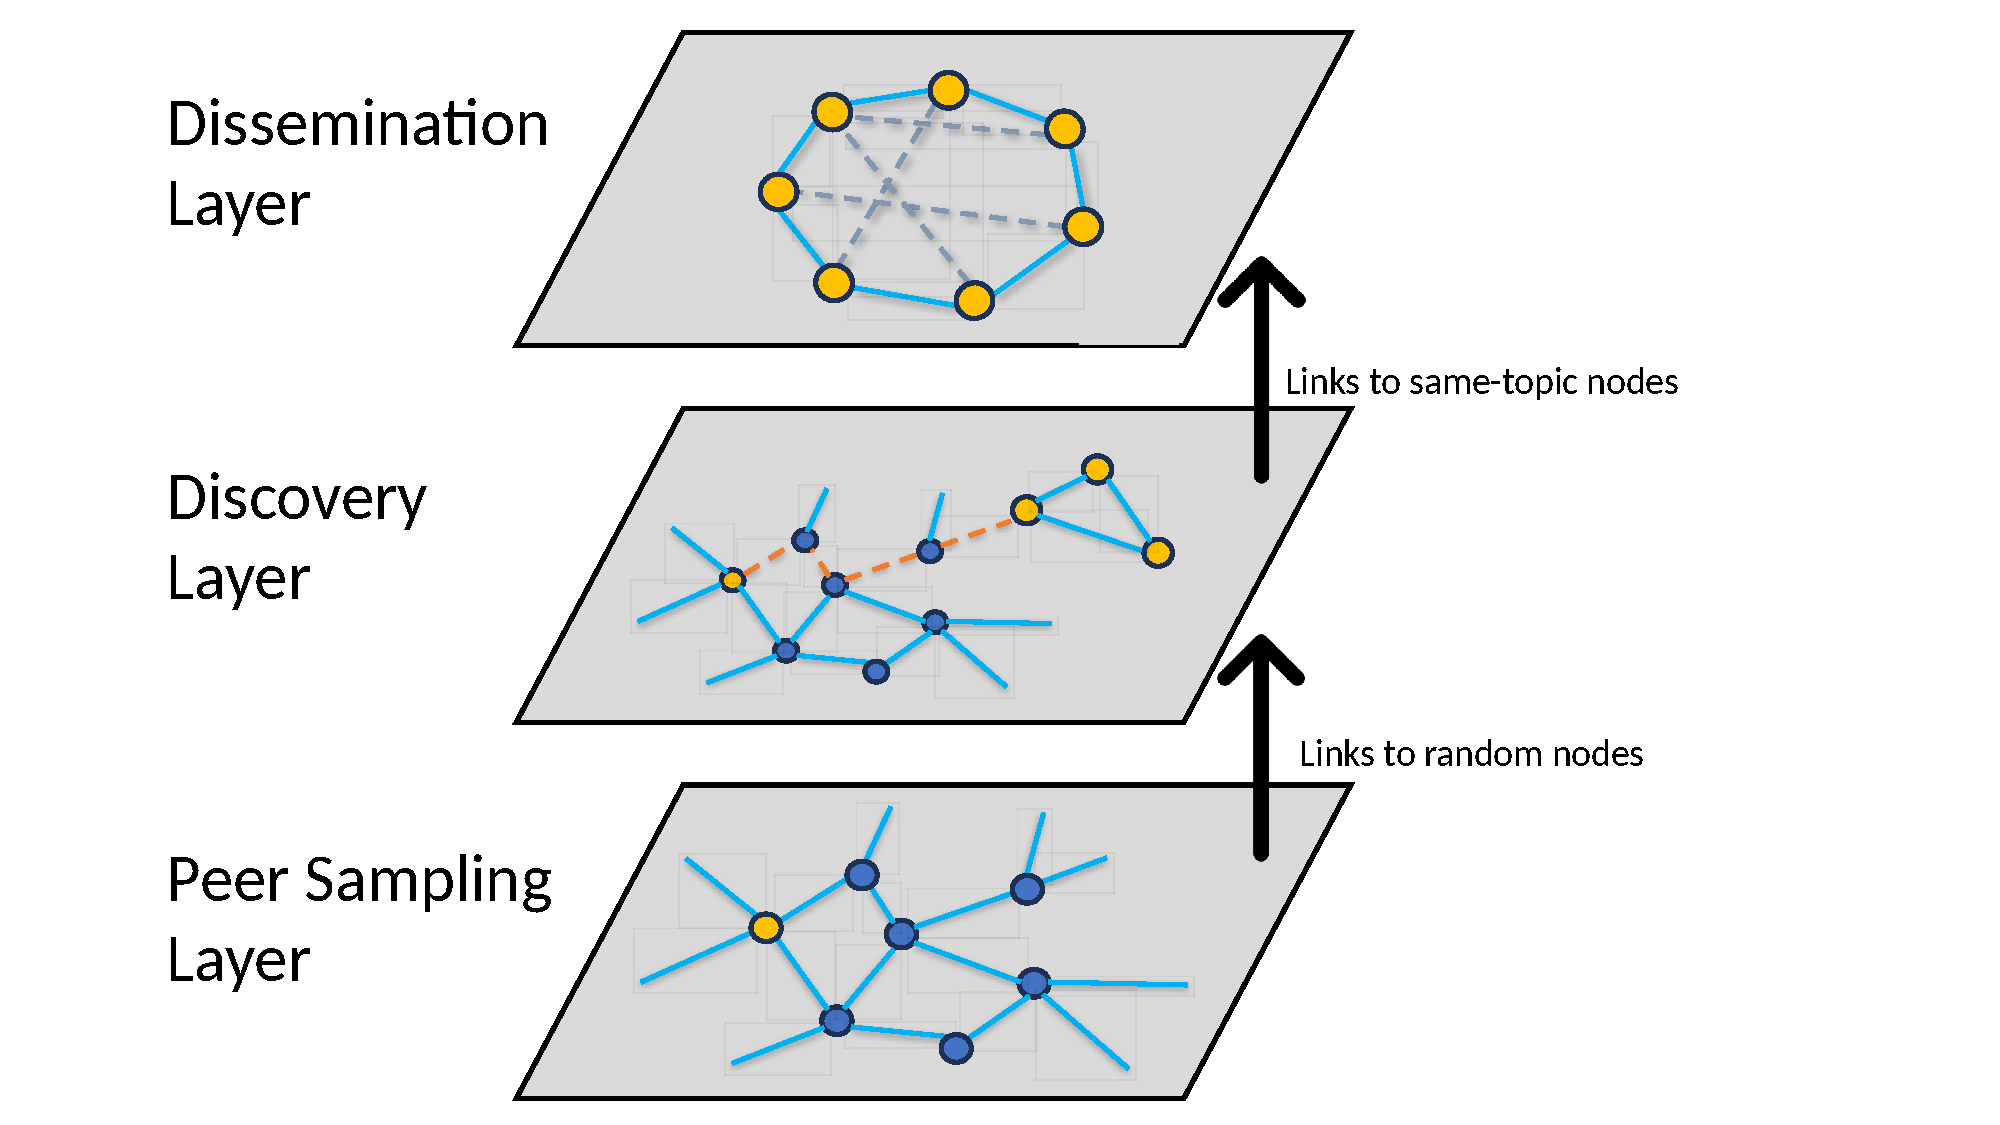
\includegraphics[width=\textwidth]{figs/layers}
        \caption{Three-layer protocol. Each layer constitutes a distinct gossiping protocol, maintaining its own list of neighbors and gossiping with them. Lower layers help higher layers by equipping them with links from their own neighbors.}
        \label{fig:dissemination_layers}
    \end{minipage}\hfill
\end{figure}

A pub/sub system encompasses a number of topics, each having its own set of subscribers to which corresponding events should be delivered. 
Thus, applying the P2P dissemination model in a pub/sub setting entails establishing one individual dissemination overlay per topic, 
as well as a global network structure combining all these overlays.
This global network structure should allow a newly joining node that contacts any arbitrary peer in it to easily and reliably discover the individual overlay(s) of the specific topic(s) it wishes to join, and
should let it participate in event dissemination therein.

Building the overlay for event dissemination is a three-faceted process.
We address it by deploying three distinct gossiping protocols, depicted as three layers in \figref{fig:dissemination_layers}.

\subsubsection{Dissemination Layer}

In order to satisfy both reliability and efficiency requirements, we adopt the dissemination algorithm proposed in Hybrid Dissemination~\cite{HybridDissemination}.
Hybrid Dissemination decouples these two fundamental goals by combining a number of random links among nodes for efficiency with a Harary graph
topology for reliability.

In Hybrid Dissemination, each node maintains a small number of $f$ links to random other nodes subscribed to the same topic.
When a node generates a new message or receives one it has not previously seen, it forwards it to all its $f$ neighbors, without
sending it back to the neighbor it received it from.
Value $f$ is a system-wide parameter, called the \emph{fanout}.
This algorithm is very efficient at spreading messages to a considerable percentage of the nodes very fast, specifically at exponential
speed with base $f$.
However, it does not guarantee that every single node will receive the message, even in the absence of failures, as a directed random graph is not necessarily strongly connected.

In order to make message dissemination reliable, Hybrid Dissemination also utilizes a Harary graph structure.
A Harary graph of $n$ nodes and connectivity $t$, denoted   $H_{t,n}$, is a minimal link graph that is guaranteed to remain connected when up to $t-1$ nodes or links fail.
In Harary graphs, links are equally distributed across all nodes, each node maintaining exactly $t$ bidirectional links to its neighbors.
These links guarantee connectivity of all nodes in a single strongly connected component.
However, dissemination over the Harary graph alone is slow, as a message has to traverse the topology sequentially.

To guarantee both efficiency and reliability in event dissemination, we combine both random links and the Harary graph structure.
In its most lightweight version, we employ a Harary graph of connectivity two, which essentially is a ring topology, and establish just one random link per node.
When a node receives a message from one of its two ring links, it forwards it to its other ring link as well as to its random link.
When a node receives a message through its random link, it forwards it along both ring links.
This uses a very low   fanout of two, while still achieving fast dissemination in a logarithmic number of steps and providing a high degree of resilience to failures, as shown in~\cite{HybridDissemination}.

%In the face of failures, the ring structure may be broken into a number of disconnected components.
%Intuitively, the use of random links delivers a message to each component with very high probability, while the use of ring links guarantees that a message will traverse all nodes of a component, up to the very last one.

\subsection{Peer Sampling Layer}
\label{subsec:peer-sampling-layer}

The Peer Sampling layer serves two primary functions.
First, it ensures that the entire set of nodes remains connected in a single connected component.
Second, it constitutes a continuous source of random peer samples, that is, fresh links to randomly chosen peers among all alive nodes in the network.
The continuous link provision ensures the systematic replacement of old---and possibly obsolete---links by newly acquired, fresh links.
This is key to peer sampling~\cite{PeerSampling}.

To satisfy these requirements, we adopt SecureCyclon~\cite{SecureCyclon}, a secure variant of the Cyclon~\cite{Cyclon} peer sampling protocol.
Cyclon is highly scalable and lightweight in network resources, as each node is only required to retain a small, fixed-sized view and to engage in small gossip exchanges once per cycle, irrespective of the network size.
SecureCyclon enforces nodes to strictly follow the gossip-exchange rules.
Specifically, it mandates that every node periodically generates only a limited number of fresh links, preventing malicious nodes from flooding the network with links to themselves and inhibiting the formation of hubs by adversaries.

As shown in~\cite{Cyclon}, Cyclon exhibits extreme robustness to node failures, self-healing properties, and uniform random peer selection, which are consequently inherited by SecureCyclon too. These properties render SecureCyclon a highly suitable substrate layer for our protocol, offering a reliable groundwork for the construction of the other two layers.